\documentclass{beamer}

\usepackage{amsmath}

\newcommand{\ind}{\perp\!\!\!\!\perp}

\usetheme{AnnArbor}
\usecolortheme{crane}
\usefonttheme[onlymath]{serif}

\title{Deep Learning - Foundations and Concepts}
\subtitle{Chapter 11. Structured Distributions}
\author{nonlineark@github}
\date{\today}

\begin{document}

\begin{frame}
    \titlepage
\end{frame}

\begin{frame}
    \frametitle{Outline}
    \tableofcontents
\end{frame}

\section{Graphical Models}

\begin{frame}
    \frametitle{Graphical models}
    The framework of probabilistic graphical models allows structured probability distributions to be expressed in graphical form:
    \begin{itemize}
        \item They provide a simple way to visualize the structure of a probabilistic model and can be used to design and motivate new models.
        \item Insights into the properties of the model, including conditional independence properties, can be obtained by inspecting the graph.
        \item The complex computations required to perform inference and learning in sophisticated models can be expressed in terms of graphical operations.
    \end{itemize}
\end{frame}

\begin{frame}
    \frametitle{Directed graphs}
    \begin{itemize}
        \item In a probabilistic graphical model, each node represents a random variable, and the links express probabilistic relationships between these variables.
        \item Directed graphical models (Bayesian networks, or Bayes nets): The graphs have a particular direction indicated by arrows, useful for expressing causal relationships between random variables (the focus of this chapter).
        \item Undirected graphical models (Markov random fields): The links do not carry arrows and have no directional significance, useful for expressing soft constraints between random variables.
    \end{itemize}
\end{frame}

\begin{frame}
    \frametitle{Factorization}
    Consider a joint distribution $p(a,b,c)$ over three variables $a$, $b$ and $c$. We can write the joint distribution in the form:
    \begin{equation*}
        p(a,b,c)=p(c|a,b)p(b|a)p(a)
    \end{equation*}
    which can be represented in terms of a simple graphical model as follows:
    \begin{itemize}
        \item Introduce a node for each of the random variables $a$, $b$ and $c$.
        \item If a random variable $y$ is conditioned on another random variable $x$, then add a directed link from $x$ to $y$. We say that $x$ is the parent of $y$, and $y$ is the child of $x$.
    \end{itemize}
\end{frame}

\begin{frame}
    \frametitle{Factorization}
    \begin{figure}
        \caption{A directed graphical model representing the decomposition $p(a,b,c)=p(c|a,b)p(b|a)p(a)$}
        \includegraphics{Figure_1.pdf}
    \end{figure}
\end{frame}

\begin{frame}
    \frametitle{Factorization}
    A directed graph also defines a joint distribution given by the product, over all of the nodes of the graph, of a conditional distribution for each node conditioned on the variables corresponding to the parents of that node in the graph. Thus for a graph with $K$ nodes, the joint distribution is given by:
    \begin{equation*}
        p(x_{1},\hdots,x_{K})=\prod_{k=1}^{K}p(x_{k}|\mathrm{pa}(k))
    \end{equation*}
    where $\mathrm{pa}(k)$ denotes the set of parents of $x_{k}$.
\end{frame}

\begin{frame}
    \frametitle{Factorization}
    \begin{figure}
        \caption{This directed graph represents the joint distribution $p(x_{1})p(x_{2})p(x_{3})p(x_{4}|x_{1},x_{2},x_{3})p(x_{5}|x_{1},x_{3})p(x_{6}|x_{4})p(x_{7}|x_{4},x_{5})$}
        \includegraphics{Figure_2.pdf}
    \end{figure}
\end{frame}

\begin{frame}
    \frametitle{Discrete variables}
    Dropping links in the graph reduces the number of independent parameters in a model. Consider two discrete variables $x^{1}$ and $x^{2}$, each of which has $K$ states. The joint distribution can be written:
    \begin{equation*}
        p(x_{1},x_{2};\mu)=\prod_{k=1}^{K}\prod_{k'=1}^{K}\mu_{kk'}^{x^{1}_{k}x^{2}_{k'}}
    \end{equation*}
    \begin{itemize}
        \item If there is a link from $x^{1}$ to $x^{2}$, we need $K^{2}-1$ parameters.
        \item If $x^{1}$ and $x^{2}$ are independent, we only need $2(K-1)$ paramters.
        \item In general, when there are $M$ variables:
        \begin{itemize}
            \item If their joint distribution is fully connected, we need $K^{M}-1$ parameters.
            \item If they are independent, we only need $M(K-1)$ parameters.
        \end{itemize}
    \end{itemize}
\end{frame}

\begin{frame}
    \frametitle{Discrete variables}
    \begin{figure}
        \caption{By dropping the link from $x^{1}$ to $x^{2}$, the number of parameters needed dropped from $K^{2}-1$ to $2(K-1)$}
        \includegraphics[trim=0 0 -1cm 0]{Figure_3_a.pdf}
        \includegraphics[trim=-1cm 0 0 0]{Figure_3_b.pdf}
    \end{figure}
\end{frame}

\begin{frame}
    \frametitle{Discrete variables}
    An alternative way to reduce the number of independent parameters in a model is by sharing parameters:
    \begin{itemize}
        \item For the graphical model on the left, we need $K-1+(M-1)K(K-1)$ parameters.
        \item For the graphical model on the right, we only need $K-1+K(K-1)=K^{2}-1$ paramters.
    \end{itemize}
    \begin{figure}
        \includegraphics[width=0.4\textwidth, trim=0 0 -1cm 0]{Figure_4.pdf}
        \includegraphics[width=0.4\textwidth, trim=-1cm 0 0 0]{Figure_5.pdf}
    \end{figure}
\end{frame}

\begin{frame}
    \frametitle{Discrete variables}
    Another way to reduce the number of independent parameters in a model is by using parameterized representations for the conditional distributions instead of complete tables of conditional probability values. For the example graph, assuming $x_{m}$ are binary variables:
    \begin{itemize}
        \item If using complete tables, we need $2^{M}$ parameters.
        \item If using parameterized representation $p(y=1|x_{1},\hdots,x_{M})=\sigma(w_{0}+\sum_{m=1}^{M}w_{m}x_{m})$, we only need $M+1$ parameters.
    \end{itemize}
    \begin{figure}
        \includegraphics{Figure_6.pdf}
    \end{figure}
\end{frame}

\begin{frame}
    \frametitle{Gaussian variables}
    For graphical models in which the nodes represent continuous variables having Gaussian distributions, we consider linear Gaussian models:
    \begin{equation*}
        p(x_{i}|\mathrm{pa}(i))=\mathcal{N}(x_{i};\sum_{j\in\mathrm{pa}(i)}w_{ij}x_{j}+b_{i},v_{i})
    \end{equation*}
    where $w_{ij}$ and $b_{i}$ are parameters governing the mean and $v_{i}$ is the variance of the conditional distribution for $x_{i}$. It's easy to see that the joint distribution is a multivariate Gaussian:
    \begin{align*}
        &-\log{}p(x_{1},\hdots,x_{D})=-\log\prod_{i=1}^{D}p(x_{i}|\mathrm{pa}(i)) \\
        &=\frac{1}{2}\sum_{i=1}^{D}\frac{1}{v_{i}}(x_{i}-\sum_{j\in\mathrm{pa}(i)}w_{ij}x_{j}-b_{i})^{2}+\frac{1}{2}\sum_{i=1}^{D}\log{}v_{i}+\frac{D}{2}\log{}2\pi
    \end{align*}
\end{frame}

\begin{frame}
    \frametitle{Gaussian variables}
    Let's calculate $E(x_{i})$ and $\mathrm{cov}(x_{i},x_{j})$:
    \begin{align*}
        E(x_{i})&=\int{}x_{i}p(x)\mathrm{d}x=\int{}x_{i}\prod_{k=1}^{D}p(x_{k}|\mathrm{pa}(k))\mathrm{d}x \\
        &=\int\prod_{k=1}^{i-1}p(x_{k}|\mathrm{pa}(k))(\int{}x_{i}p(x_{i}|\mathrm{pa}(i))\mathrm{d}x_{i})\mathrm{d}x_{1}\cdots\mathrm{d}x_{i-1} \\
        &=\int(\sum_{j\in\mathrm{pa}(i)}w_{ij}x_{j}+b_{i})\prod_{k=1}^{i-1}p(x_{k}|\mathrm{pa}(k))\mathrm{d}x_{1}\cdots\mathrm{d}x_{i-1} \\
        &=\int(\sum_{j\in\mathrm{pa}(i)}w_{ij}x_{j}+b_{i})p(x)\mathrm{d}x \\
        &=\sum_{j\in\mathrm{pa}(i)}w_{ij}E(x_{j})+b_{i}
    \end{align*}
\end{frame}

\begin{frame}
    \frametitle{Gaussian variables}
    For $i<j$:
    \begin{align*}
        E(x_{i}x_{j})&=\int{}x_{i}x_{j}p(x)\mathrm{d}x=\int{}x_{i}x_{j}\prod_{l=1}^{D}p(x_{l}|\mathrm{pa}(l))\mathrm{d}x \\
        &=\int{}x_{i}\prod_{l=1}^{j-1}p(x_{l}|\mathrm{pa}(l))(\int{}x_{j}p(x_{j}|\mathrm{pa}(j))\mathrm{d}x_{j})\mathrm{d}x_{1}\cdots\mathrm{d}x_{j-1} \\
        &=\int(\sum_{k\in\mathrm{pa}(j)}w_{jk}x_{k}+b_{j})x_{i}\prod_{l=1}^{j-1}p(x_{l}|\mathrm{pa}(l))\mathrm{d}x_{1}\cdots\mathrm{d}x_{j-1} \\
        &=\int(\sum_{k\in\mathrm{pa}(j)}w_{jk}x_{k}+b_{j})x_{i}p(x)\mathrm{d}x \\
        &=\sum_{k\in\mathrm{pa}(j)}w_{jk}E(x_{i}x_{k})+b_{j}E(x_{i})
    \end{align*}
\end{frame}

\begin{frame}
    \frametitle{Gaussian variables}
    \begin{align*}
        E(x_{i}^{2})&=\int{}x_{i}^{2}p(x)\mathrm{d}x=\int{}x_{i}^{2}\prod_{l=1}^{D}p(x_{l}|\mathrm{pa}(l))\mathrm{d}x \\
        &=\int\prod_{l=1}^{i-1}p(x_{l}|\mathrm{pa}(l))(\int{}x_{i}^{2}p(x_{i}|\mathrm{pa}(i))\mathrm{d}x_{i})\mathrm{d}x_{1}\cdots\mathrm{d}x_{i-1} \\
        &=\int((\sum_{k\in\mathrm{pa}(i)}w_{ik}x_{k}+b_{i})^{2}+v_{i})\prod_{l=1}^{i-1}p(x_{l}|\mathrm{pa}(l))\mathrm{d}x_{1}\cdots\mathrm{d}x_{i-1} \\
        &=\int((\sum_{k\in\mathrm{pa}(i)}w_{ik}x_{k}+b_{i})^{2}+v_{i})p(x)\mathrm{d}x \\
        &=\sum_{j,k\in\mathrm{pa}(i)}w_{ij}w_{ik}E(x_{j}x_k)+2b_{i}\sum_{k\in\mathrm{pa}(i)}w_{ik}E(x_{k})+b_{i}^{2}+v_{i}
    \end{align*}
\end{frame}

\begin{frame}
    \frametitle{Gaussian variables}
    Finally, for $i\ne{}j$ we have:
    \begin{align*}
        \mathrm{cov}(x_{i},x_{j})&=E(x_{i}x_{j})-E(x_{i})E(x_{j})=\sum_{k\in\mathrm{pa}(j)}w_{jk}\mathrm{cov}(x_{i},x_{k}) \\
        \mathrm{cov}(x_{i},x_{i})&=E(x_{i}^{2})-(E(x_{i}))^{2} \\
        &=\sum_{j,k\in\mathrm{pa}(i)}w_{ij}w_{ik}\mathrm{cov}(x_{j},x_{k})+v_{i} \\
        &=\sum_{k\in\mathrm{pa}(i)}w_{ik}\mathrm{cov}(x_{i},x_{k})+v_{i}
    \end{align*}
    We can calculate $E(x_{i})$ and $\mathrm{cov}(x_{i},x_{j})$ by starting at the lowest numbered node and working recursively through the graph.
\end{frame}

\begin{frame}
    \frametitle{Binary classifier}
    Suppose a binary classifier model has probability distributions of the form:
    \begin{align*}
        &p(t_{1},\hdots,t_{N},w|x^{1},\hdots,x^{N};\lambda)=p(w;\lambda)\prod_{n=1}^{N}p(t_{n}|x^{n};w) \\
        &p(w;\lambda)=\mathcal{N}(w;0,\lambda{}I)
    \end{align*}
    \begin{figure}
        \caption{Directed graphical model representing the binary classifier model and its more compact version}
        \includegraphics[trim=0 0 -1cm 0]{Figure_8.pdf}
        \includegraphics[trim=-1cm 0 0 0]{Figure_9.pdf}
    \end{figure}
\end{frame}

\begin{frame}
    \frametitle{Parameters and observations}
    There are three kinds of variables in a directed graphical model:
    \begin{itemize}
        \item Unobserved (also called latent, or hidden) stochastic variables are denoted by open red circles.
        \item When stochastic variables are observed, so that they are set to specific values, they are denoted by red circles shaded with blue.
        \item Non-stochastic parameters are denoted by floating variables.
    \end{itemize}
    \begin{figure}
        \includegraphics{Figure_11.pdf}
    \end{figure}
\end{frame}

\begin{frame}
    \frametitle{Bayes' theorem}
    \begin{figure}
        \caption{A graphical representation of Bayes' theorem}
        \includegraphics[trim=0 0 -1cm 0]{Figure_13_a.pdf}
        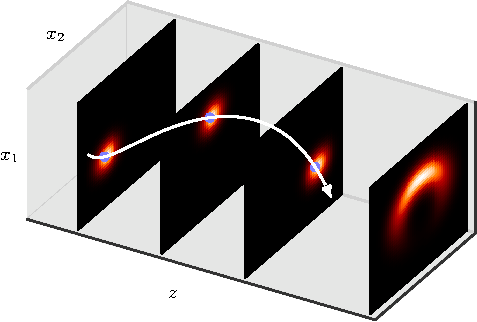
\includegraphics[trim=-1cm 0 -1cm 0]{Figure_13_b.pdf}
        \includegraphics[trim=-1cm 0 0 0]{Figure_13_c.pdf}
    \end{figure}
\end{frame}

\section{Conditional Independence}

\begin{frame}
    \frametitle{Conditional independence}
    Consider three variables $a$, $b$ and $c$, we say that $a$ is conditionally independent of $b$ given $c$ if
    \begin{equation*}
        p(a|b,c)=p(a|c)
    \end{equation*}
    holds for every possible value of $c$. Equivalently, this can be written as:
    \begin{equation*}
        p(a,b|c)=p(a|b,c)p(b|c)=p(a|c)p(b|c)
    \end{equation*}
    We will sometimes use a shorthand notation for conditional independence in which
    \begin{equation*}
        a\ind{}b|c
    \end{equation*}
    denotes that $a$ is conditionally independent of $b$ given $c$. In particular, the notation $a\ind{}b|\emptyset$ denotes that $a$ is independent of $b$.
\end{frame}

\begin{frame}
    \frametitle{Conditional independence}
    \begin{itemize}
        \item An important and elegant feature of graphical models is that conditional independence properties of the joint distribution can be read directly from the graph without having to perform any analytical manipulations.
        \item The general framework for achieving this is called d-separation, where the ``d'' stands for ``directed''.
    \end{itemize}
\end{frame}

\begin{frame}
    \frametitle{Three example graphs}
    \begin{figure}
        \caption{The first of three examples}
        \includegraphics[trim=0 0 -1cm 0]{Figure_14.pdf}
        \includegraphics[trim=-1cm 0 0 0]{Figure_15.pdf}
    \end{figure}
\end{frame}

\begin{frame}
    \frametitle{Three example graphs}
    \begin{itemize}
        \item The joint distribution is given by: $p(a,b,c)=p(a|c)p(b|c)p(c)$.
        \begin{itemize}
            \item Question: Is $a\ind{}b|\emptyset$ true?
            \item Answer: No, because $p(a,b)=\sum_{c}p(a,b,c)=\sum_{c}p(a|c)p(b|c)p(c)\ne{}p(a)p(b)$.
            \item Question: Is $a\ind{}b|c$ true?
            \item Answer: Yes, because $p(a,b|c)=\frac{p(a,b,c)}{p(c)}=p(a|c)p(b|c)$.
        \end{itemize}
        \item Consider the path from node $a$ to node $b$ via $c$:
        \begin{itemize}
            \item The node $c$ is said to be tail-to-tail with respect to this path.
            \item The presence of such a path connecting nodes $a$ and $b$ causes these nodes to be dependent.
            \item The conditioned node blocks the path from $a$ to $b$ and causes $a$ and $b$ to become conditionally independent.
        \end{itemize}
    \end{itemize}
\end{frame}

\begin{frame}
    \frametitle{Three example graphs}
    \begin{figure}
        \caption{The second of three examples}
        \includegraphics[trim=0 0 -1cm 0]{Figure_16.pdf}
        \includegraphics[trim=-1cm 0 0 0]{Figure_17.pdf}
    \end{figure}
\end{frame}

\begin{frame}
    \frametitle{Three example graphs}
    \begin{itemize}
        \item The joint distribution is given by: $p(a,b,c)=p(a)p(b|c)p(c|a)$.
        \begin{itemize}
            \item Question: Is $a\ind{}b|\emptyset$ true?
            \item Answer: No, because $p(a,b)=\sum_{c}p(a,b,c)=\sum_{c}p(a)p(b|c)p(c|a)\ne{}p(a)p(b)$.
            \item Question: Is $a\ind{}b|c$ true?
            \item Answer: Yes, because $p(a,b|c)=\frac{p(a,b,c)}{p(c)}=p(a|c)p(b|c)$.
        \end{itemize}
        \item Consider the path from node $a$ to node $b$ via $c$:
        \begin{itemize}
            \item The node $c$ is said to be head-to-tail with respect to this path.
            \item The presence of such a path connecting nodes $a$ and $b$ causes these nodes to be dependent.
            \item The conditioned node blocks the path from $a$ to $b$ and causes $a$ and $b$ to become conditionally independent.
        \end{itemize}
    \end{itemize}
\end{frame}

\begin{frame}
    \frametitle{Three example graphs}
    \begin{figure}
        \caption{The third of three examples}
        \includegraphics[trim=0 0 -1cm 0]{Figure_18.pdf}
        \includegraphics[trim=-1cm 0 0 0]{Figure_19.pdf}
    \end{figure}
\end{frame}

\begin{frame}
    \frametitle{Three example graphs}
    \begin{itemize}
        \item The joint distribution is given by: $p(a,b,c)=p(a)p(b)p(c|a,b)$.
        \begin{itemize}
            \item Question: Is $a\ind{}b|\emptyset$ true?
            \item Answer: Yes, because $p(a,b)=\sum_{c}p(a,b,c)=\sum_{c}p(a)p(b)p(c|a,b)=p(a)p(b)$.
            \item Question: Is $a\ind{}b|c$ true?
            \item Answer: No, because $p(a,b|c)=\frac{p(a,b,c)}{p(c)}\ne{}p(a|c)p(b|c)$.
        \end{itemize}
        \item Consider the path from node $a$ to node $b$ via $c$:
        \begin{itemize}
            \item The node $c$ is said to be head-to-head with respect to this path.
            \item When node $c$ is unobserved, it blocks the path, and the variables $a$ and $b$ are independent.
            \item Conditioning on $c$ unblocks the path and renders $a$ and $b$ dependent. In fact, a head-to-head path will become unblocked if either the node, or any of its descendants, is observed.
        \end{itemize}
    \end{itemize}
\end{frame}

\begin{frame}
    \frametitle{Explaining away}
    To understand further the unusual behavior of the third example, consider three binary random variables relating to the fuel system on a car:
    \begin{itemize}
        \item $B$: The state of a battery that is either charged ($B=1$) or flat ($B=0$).
        \item $F$: The state of the fuel tank that is either full of fuel ($F=1$) or empty ($F=0$).
        \item $G$: The state of an electric fuel gauge and which indicates that the fuel tank is either full ($G=1$) or empty ($G=0$).
    \end{itemize}
    \begin{figure}
        \includegraphics{Figure_20.pdf}
    \end{figure}
\end{frame}

\begin{frame}
    \frametitle{Explaining away}
    And here is the probability table:
    \begin{align*}
        &p(B=1)=0.9 \\
        &p(F=1)=0.9 \\
        &p(G=1|F=1,B=1)=0.8 \\
        &p(G=1|F=1,B=0)=0.2 \\
        &p(G=1|F=0,B=1)=0.2 \\
        &p(G=1|F=0,B=0)=0.1
    \end{align*}
    Let's calculate $p(F=0|G=0)$ and $p(F=0|G=0,B=0)$.
\end{frame}

\begin{frame}
    \frametitle{Explaining away}
    \begin{align*}
        p(F=0)&=0.1 \\
        p(F=0|G=0)&=\frac{p(F=0,G=0)}{p(G=0)} \\
        &=\frac{0.072+0.009}{0.162+0.072+0.072+0.009}=\frac{9}{35}\approx{}0.257 \\
        p(F=0|G=0,B=0)&=\frac{p(F=0,G=0,B=0)}{p(G=0,B=0)} \\
        &=\frac{0.009}{0.072+0.009}=\frac{1}{9}\approx{}0.111
    \end{align*}
\end{frame}

\begin{frame}
    \frametitle{Explaining away}
    \begin{itemize}
        \item We see that $p(F=0|G=0)\ne{}p(F=0|G=0,B=0)$, which means, when $G$ is observed, $F$ and $B$ are indeed dependent.
        \item This accords with our intuition that finding that the battery is flat explains away the observation that the fuel gauge reads empty.
        \item In fact, this would also be the case if, instead of observing the fuel gauge directly, we observed the state of some descendant of $G$, for example a rather unreliable witness who reports seeing that the gauge was reading empty.
    \end{itemize}
\end{frame}

\begin{frame}
    \frametitle{D-separation}
    Consider a general directed graph in which $A$, $B$ and $C$ are arbitrary non-intersecting sets of nodes. To determine whether a particular conditional independence statement $A\ind{}B|C$ is true, we consider all possible paths from any node in $A$ to any node in $B$. Any such path is said to be blocked if it includes a node such that either:
    \begin{itemize}
        \item The arrows on the path meet either head-to-tail or tail-to-tail at the node, and the node is in the set $C$.
        \item The arrows meet head-to-head at the node and neither the node, nor any of its descendants is in the set $C$.
    \end{itemize}
    If all paths are blocked, then $A$ is said to be d-separated from $B$ by $C$, and the joint distribution over all the variables in the graph will satisfy $A\ind{}B|C$.
\end{frame}

\begin{frame}
    \frametitle{Naive Bayes}
    Suppose we wish to assign values of $x$ to one of $K$ classes. The key assumption of the naive Bayes model is that, conditioned on the class $\mathcal{C}_{k}$, the distribution of the input variable factorizes into the product of two or more densities. Suppose we partition $x$ into $L$ elements $x=(x^{(1)},\hdots,x^{(L)})$, naive Bayes then takes the form:
    \begin{equation*}
        p(x|\mathcal{C}_{k})=\prod_{l=1}^{L}p(x^{(l)}|\mathcal{C}_{k})
    \end{equation*}
    It is assumed that this holds for each of the classes $\mathcal{C}_{k}$ separately.
    \begin{figure}
        \includegraphics{Figure_22.pdf}
    \end{figure}
\end{frame}

\begin{frame}
    \frametitle{Generative models}
    \begin{itemize}
        \item Discriminative model: Take an image as input and generate outputs that describe the object's class, position and scale.
        \item Generative model: Select values for object's class, postion and scale from the learned prior distributions and then subsequently sampling an image from the learned conditional distribution.
    \end{itemize}
    \begin{figure}
        \includegraphics{Figure_24.pdf}
    \end{figure}
\end{frame}

\begin{frame}
    \frametitle{Markov blanket}
    Consider a joint distribution $p(x_{1},\hdots,x_{D})$ represented by a directed graph having $D$ nodes, and consider the conditional distribution of a particular node $x_{i}$ conditioned on all the remaining nodes $x_{j\ne{}i}$:
    \begin{equation*}
        p(x_{i}|x_{j\ne{}i})=\frac{p(x_{1},\hdots,x_{D})}{\int{}p(x_{1},\hdots,x_{D})\mathrm{d}x_{i}}=\frac{\prod_{d=1}^{D}p(x_{d}|\mathrm{pa}(d))}{\int\prod_{d=1}^{D}p(x_{d}|\mathrm{pa}(d))\mathrm{d}x_{i}}
    \end{equation*}
    The only factors that remain will be:
    \begin{itemize}
        \item $p(x_{i}|\mathrm{pa}(i))$.
        \item $p(x_{d}|\mathrm{pa}(d))$ if $i\in\mathrm{pa}(d)$.
    \end{itemize}
\end{frame}

\begin{frame}
    \frametitle{Markov blanket}
    We can think of the Markov blanket of a node $x_{i}$ as being the minimal set of nodes that isolates $x_{i}$ from the rest of the graph, which comprises of:
    \begin{itemize}
        \item The parents, from factor $p(x_{i}|\mathrm{pa}(i))$.
        \item The children, from factor $p(x_{d}|\mathrm{pa}(d))$.
        \item The co-parents, from factor $p(x_{d}|\mathrm{pa}(d))$.
    \end{itemize}
    \begin{figure}
        \includegraphics{Figure_25.pdf}
    \end{figure}
\end{frame}

\begin{frame}
    \frametitle{Graphs as filters}
    A directed graph:
    \begin{itemize}
        \item Represents a specific decomposition of a joint probability distribution into a product of conditional probabilities.
        \item Expresses a set of conditional independence statements obtained through the d-separation criterion.
    \end{itemize}
    These two properties are equivalent. If we present to the graph the set of all possible distributions $p(x)$:
    \begin{itemize}
        \item Graph as a joint distribution filter: The subset of distributions that can be expressed in terms of the factorization implied by the graph is denoted $\mathcal{DF}_{1}$.
        \item Graph as a conditional independence filter: The subset of distributions that satisfy all the conditional independence properties obtained by applying the d-separation criterion to the graph is denoted $\mathcal{DF}_{2}$.
    \end{itemize}
    Then the d-separation theorem tells us that $\mathcal{DF}_{1}=\mathcal{DF}_{2}$.
\end{frame}

\end{document}